\documentclass[11pt]{article}

\usepackage{extras} % Se extras.sty

\begin{document}
\begin{titlepage}
\begin{center}

{\Large\bfseries TSEA56 - Kandidatprojekt i elektronik \\ LIPS Designspecifikation}

\vspace{5em}

Version 0.1

\vspace{5em}
Grupp 4 \\
\begin{tabular}{rl}
Hynén Ulfsjöö, Olle&\verb+ollul666+
\\
Wasteson, Emil&\verb+emiwa068+
\\
Tronje, Elena&\verb+eletr654+
\\
Gustafsson, Lovisa&\verb+lovgu777+
\\
Inge, Zimon&\verb+zimin415+
\\
Strömberg, Isak&\verb+isast763+
\\
\end{tabular}

\vspace{5em}
\today

\vspace{16em}
Status
\begin{longtable}{|l|l|l|} \hline

Granskad & - & - \\ \hline
Godkänd & - & - \\ \hline
 
\end{longtable}

\end{center}
\end{titlepage}

\pagebreak
\begin{center}

\section*{PROJEKTIDENTITET}
2016/VT, Undsättningsrobot Gr. 4

Linköpings tekniska högskola, ISY
\vspace{5em}
%\begin{center}

\begin{tabular}{|l|l|l|l|} \hline
\textbf{Namn} & \textbf{Ansvar} & \textbf{Telefon} & \textbf{E-post}  \\ \hline 
Isak Strömberg (IS) & Projektledare & 073-980 38 50 & isast763@student.liu.se \\ \hline
Olle Hynén Ulfsjöö (OHU)& Dokumentansvarig & 070-072 91 84 & ollul666@student.liu.se \\ \hline
Emil Wasteson (EW) & Hårdvaruansvarig & 076-836 61 66 & emiwa068@student.liu.se \\ \hline
Elena Tronje (ET) & Mjukvaruansvarig & 072-276 92 93 & eletr654@student.liu.se \\ \hline
Zimon Inge (ZI)& Testansvarig & 070-171 35 18 & zimin415@student.liu.se \\ \hline
Lovisa Gustafsson (LG) & Leveransansvarig & 070-210 32 53 & lovgu777@student.liu.se \\ \hline
\end{tabular}

%\end{center}

E-postlista för hela gruppen: isast763@student.liu.se

\vspace{5em}
Kund: ISY, Linköpings universitet 
tel: 013-28 10 00, fax: 013-13 92 82 \\
Kontaktperson hos kund: Mattias Krysander \\
tel: 013-28 21 98, e-post: matkr@isy.liu.se \\

\vspace{5em}
Kursansvarig:  Tomas Svensson\\
tel: 013-28 13 68, e-post: tomass@isy.liu.se \\
Handledare: Peter Johansson \\
tel: 013-28 13 45, e-post: peter.a.johansson@liu.se
\end{center}
\pagebreak

\tableofcontents

\pagebreak

\section*{Dokumenthistorik}
\begin{table}[h]
\begin{tabular}{|l|l|l|l|l|} \hline

\textbf{Version} & \textbf{Datum} & \textbf{Utförda förändringar} & \textbf{Utförda av} & \textbf{Granskad} \\ \hline
0.1 & - &  Första utkastet & Grupp 4 & - \\ \hline
\end{tabular}
\end{table}

\pagebreak
\pagenumbering{arabic}

\begin{flushleft}
\section{Inledning}
\lipsum

\subsection{Det totala systemet}
Det totala system kommer bestå av tre processormoduler, en Bluetooth\textsuperscript{\circledR}, ett chassi med inbyggda motorer, en gripklo, ett styrservo och ett antal olika sensorer. De olika modulerna är:
\begin{itemize}
	\item Huvudmodul - sköter kommunikationen, både internt via I\textsuperscript{2}C-bussen och externt via en Bluetooth\textsuperscript{\circledR}-enhet.
	\item Sensormodul - är direkt kopplad till alla sensor och tar emot och konverterar all data från dessa (främst i form av analoga spänningar). Den färdigkonverterade datan skickas sedan vidare till huvudmodulen.
	\item Styrmodul - är sammankopplad med gripklon, ett servo för rotation av vissa sensorer och chassits motorer. Den tar emot instruktioner och data för reglering från huvudmodulen.
\end{itemize}
Förutom förbindelserna med olika externa enheter är de tre modulerna sammankopplade med en I\textsuperscript{2}C-buss, där huvudmodulen är master och kontrollerar kommunikationen. 

En övergripande bild över systemet återfinns i figur \ref{overview}.

\begin{figure}[!htbp]
\centering
\noindent\resizebox{\linewidth}{!}{
	
\documentclass[border=10px]{standalone}
\usepackage{tikz}
\usetikzlibrary{patterns}
\usetikzlibrary{shapes.arrows}
\usepackage{amssymb}
\usetikzlibrary{calc}
\usepackage{verbatim}
\usetikzlibrary{decorations.pathmorphing}

\begin{document}
	
\begin{tikzpicture}[scale=1,rotate=0]
		
	%Base
	\draw[thick, draw=black, fill=gray!10] (0,0) rectangle (6,10);

	%Wheels
	\draw[thick, pattern=north west lines, pattern color=black] (-.5,1) 		rectangle (0,2.5);
	\draw[thick, pattern=north west lines, pattern color=black] (-.5,7.5) 	rectangle (0,9);
	\draw[thick, pattern=north west lines, pattern color=black] (6,1) 		rectangle (6.5,2.5);
	\draw[thick, pattern=north west lines, pattern color=black] (6,7.5) 		rectangle (6.5,9);
	
	%Sensors
	\draw[thick, draw=black, fill=white]		(-.25,.25) 		rectangle 	(.5,.75);
	\draw[thick, draw=black, fill=white] 	(-.25,9.25) 		rectangle 	(.5,9.75);
	\draw[thick, draw=black, fill=white] 	(5.5,.25) 		rectangle 	(6.25,.75);
	\draw[thick, draw=black, fill=white] 	(5.5,9.25) 		rectangle 	(6.25,9.75);
	\draw[thick, draw=black, fill=white] 	(1.5,10.25) 		rectangle 	(4.5,9.5);
	\draw[thick, draw=black]				 	(2.5,9.5)			--		  	(2.5,10.25);
	\draw[thick, draw=black]					(3.5,9.5) --++ (0,.75);
	
	%Gripklo
	\draw[thick, draw=black, <-] (3,10.25) --++ (0,.72) node[above] {Gripklo};
	
	%Lidar lite
	\draw[thick, draw=black, <-] 			(1.5,10.25)  		--+ 		  	(135:1) node[above, align=center] {\verb+LIDAR-Lite v2+ \\ med servo};
	%Identifierare av nödställd
	\draw[thick, draw=black, <-]				(4.5,10.25)		--+			(45:1)  node[above] {\verb+IRM-8601-S+};
	
	%IR sensorer
	\draw[thick, draw=black, <-]				(-.25, 9.75) 	--+			(135:1) node[above] {\verb+GP2D120+};
	\draw[thick, draw=black, <-]				(-.25, .25) 		--+			(225:1) node[below] {\verb+GP2D120+};
	\draw[thick, draw=black, <-]				(6.25, 9.75) 	--+			(45:1) node[above] {\verb+GP2D120+};
	\draw[thick, draw=black, <-]				(6.25, .25) 		--+			(315:1) node[below] {\verb+GP2D120+};
	
	\draw[thick, draw=black, fill=white]					(2.5,4.5)		rectangle	(3.5,5.5);
	
	%Gyro
	\draw[thick, draw=black, <-] (3.5,5) --++ (.25,0) node[rotate=270, above] {\verb+MLX90609+};
	
	%Arrows and text
	%\draw[thick, ->]  (3,11) node[left, align=center] {\verb+LIDAR-Lite v2+ \\ + detektor av nödställd} -- (3,10.25);
	%\draw[thick, <->] (0.5,0.5)  --  (5.5,0.5) node[left=-14pt,midway, fill=gray!10] {\verb+GP2D120+};
	%\draw[thick, <->] (0.5,9.5) -- (3,9) node[right=-14pt,fill=gray!10] {\verb+GP2D120+} -- (5.5,9.5);
	%\draw[thick, ->] (4.5,5) node[above] {\verb+MPU-6500+} -- (3.5,5);
	
	%Sensormodul
	\node (sensormodul) at (3,6.75) [thick, draw=black, minimum width=3cm, minimum height=1.5cm, align=center, fill=white] {Sensormodul \\ \verb+ATmega1284p+};
	
	%Huvudmodul
	\node (huvudmodul) at (3,3.25) [thick, draw=black, minimum width=3cm, minimum height=1.5cm, align=center, fill=white] {Huvudmodul \\ \verb+ATmega1284p+};
	
	%Styrmodul
	\node (styrmodul) at (3,1.25) [thick, draw=black, minimum width=3cm, minimum height=1.5cm, align=center, fill=white] {Styrmodul \\ \verb+ATmega1284p+};
	
	%I2C-buss
	\draw[thick, draw=teal] ($(sensormodul.north east) + (.25,0)$) -- ($(styrmodul.south east) + (.25,0)$);
	\draw[thick, draw=teal] ($(sensormodul.north east) + (.5,0)$) -- ($(styrmodul.south east) + (.5,0)$);
	\node (i2c) at ($(sensormodul.north east) + (0.375,.25)$) [text=teal] {\small I\textsuperscript{2}C};
	
	\draw[thick, draw=teal, fill=teal] ($(sensormodul.south east) + (0,.25)$) --+ (.25,0) circle [radius=.05cm];
	\draw[thick, draw=teal, fill=teal] ($(sensormodul.south east) + (0,.5)$) --+ (.5,0) circle [radius=.05cm];
	
	\draw[thick, draw=teal, fill=teal] ($(huvudmodul.south east) + (0,.25)$) --+ (.25,0) circle [radius=.05cm];
	\draw[thick, draw=teal, fill=teal] ($(huvudmodul.south east) + (0,.5)$) --+ (.5,0) circle [radius=.05cm];
	
	\draw[thick, draw=teal, fill=teal] ($(styrmodul.south east) + (0,.25)$) --+ (.25,0) circle [radius=.05cm];
	\draw[thick, draw=teal, fill=teal] ($(styrmodul.south east) + (0,.5)$) --+ (.5,0) circle [radius=.05cm];
	
	%Koppling till sensormodul
	\draw[thick, draw=violet] (.5,9.5) --++ (.25,0) --++ (0,-2.5) --++ (0.75,0) ;
	\draw[thick, draw=violet] (.5,.5) --++ (.25,0) --++ (0,6.25) --++ (0.75,0);
	
	\draw[thick, draw=violet] (5.5,9.5) --++ (-.25,0) --++ (0,-2.5) --++ (-0.75,0);
	\draw[thick, draw=violet] (5.5,.5) --++ (-.25,0) --++ (0,6.25) --++ (-0.75,0);
	
	\draw[thick, draw=violet] (2,9.5) --++ (0,-2);
	\draw[thick, draw=violet] (4,9.5) --++ (0,-2);
	
	\draw[thick, draw=violet] (sensormodul.south) --++ (0,-.5);
	
	%Kopplingar till styrmodul
	\draw[thick, draw=olive] (styrmodul.east) --++ (1.5,0);
	\draw[thick, draw=olive] (styrmodul.west) --++ (-1.5,0);
	\draw[thick, draw=olive] ($(styrmodul.east) + (0,.25)$) --++ (1,0) --++ (0,6.25) --++ (.5,0);
	\draw[thick, draw=olive] ($(styrmodul.west) + (0,.25)$) --++ (-1,0) --++ (0,6.25) --++ (-.5,0);
	\draw[thick, draw=olive] (3,9.5) --++ (0,-1.75) --++ (-1.75,0) --++ (0,-6) --++ (.25,0);
	
	%Bluetooth
	\draw[thick, draw=black] (huvudmodul.east) --++ (2,0) node[right,minimum width=.75cm, minimum height=1cm, draw=black] (bt) {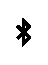
\includegraphics{bluetooth}};
	
	\node (bt2) at ($(bt) + (2,0)$) [thick, draw=black, minimum width=.75cm, minimum height=1cm] {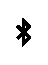
\includegraphics{bluetooth}};
	
	\draw[thick, ->,line join=round,decorate, decoration={
    												snake,
    												segment length=5,
    												amplitude=1,
    												post=lineto,
    												post length=1pt}] 
    		($(bt.east) + (5pt,5pt)$) -- ($(bt2.west) + (-5pt,5pt)$);
    		
    \draw[thick, ->,line join=round,decorate, decoration={
    												snake,
    												segment length=5,
    												amplitude=1,
    												post=lineto,
    												post length=1pt}] 
    		 ($(bt2.west) + (-5pt,-5pt)$) -- ($(bt.east) + (5pt,-5pt)$);
    		 
    \draw[thick, draw=black] (bt2.east) --++ (.5,0) node[right, minimum width=3cm, minimum height=1.5cm, draw=black, fill=white] {Datormodul};
    
    \draw[thick, draw=black] ($(sensormodul.south west) + (.25,0)$) --++ (0,-2) node[midway, above, sloped] {\small avbrott};
    
    \draw[thick, draw=black] ($(styrmodul.north west) + (.25,0)$) -- ($(huvudmodul.south west) + (.25,0)$) node[right, midway] {\small avbrott};
	
	\end{tikzpicture}
	
\end{document}  
}
	\caption{Det totala systemet \label{overview}}	
\end{figure}

\FloatBarrier
\subsection{Sensorer}
Roboten kommer vara utrustad med sex olika sensorer. Fyra infraröda sensorer av typen \verb+GP2D120+ används för att bestämma avstånden till väggarna på robotens sidor och robotens vinkel i förhållande till dessa, värden som används vid reglering av robotens rörelse rakt fram. Vidare finns ett kombinerat 3-axligt gyro och 3-axlig accelerometer av typen \verb+MPU-6500+ som används för att reglera rotation av roboten. Slutligen finns en lasersensor av typen \verb+Lidar-Lite v2+ för att bestämma avståndet till väggar framför roboten. Placeringen av sensorerna visas nedan i figur \ref{sensor}.

\begin{figure}[htbp]
\centering
\noindent\resizebox{.8\linewidth}{!}{
	\documentclass[border=10px]{standalone}
\usepackage{tikz}
\usetikzlibrary{patterns}
\usetikzlibrary{shapes.arrows}
\usepackage{amssymb}
\usetikzlibrary{calc}
\usepackage{verbatim}
\begin{document}
	
\begin{tikzpicture}[scale=1,rotate=90]
		
	%Base
	\draw[thick, draw=black, fill=gray!10] (0,0) rectangle (6,10);

	%Wheels
	\draw[thick, pattern=north west lines, pattern color=black] (-.5,1) 		rectangle (0,2.5);
	\draw[thick, pattern=north west lines, pattern color=black] (-.5,7.5) 	rectangle (0,9);
	\draw[thick, pattern=north west lines, pattern color=black] (6,1) 		rectangle (6.5,2.5);
	\draw[thick, pattern=north west lines, pattern color=black] (6,7.5) 		rectangle (6.5,9);
	
	%Sensors
	\draw[thick, draw=black, fill=white] (-.25,.25) 		rectangle (.5,.75);
	\draw[thick, draw=black, fill=white] (-.25,9.25) 	rectangle (.5,9.75);
	\draw[thick, draw=black, fill=white] (5.5,.25) 		rectangle (6.25,.75);
	\draw[thick, draw=black, fill=white] (5.5,9.25) 		rectangle (6.25,9.75);
	\draw[thick, draw=black, fill=white] (2,10.25) 		rectangle (4,9.5);
	\draw[thick, draw=black, fill=white] (2.5,4) 		rectangle (3.5,6);
	
	%Arrows and text
	\draw[thick, ->]  (3,11) node[left, align=center] {\verb+LIDAR-Lite v2+ \\ + detektor av nödställd} -- (3,10.25);
	\draw[thick, <->] (0.5,0.5)  --  (5.5,0.5) node[left=-14pt,midway, fill=gray!10] {\verb+GP2D120+};
	\draw[thick, <->] (0.5,9.5) -- (3,9) node[right=-14pt,fill=gray!10] {\verb+GP2D120+} -- (5.5,9.5);
	\draw[thick, ->] (4.5,5) node[above] {\verb+MLX90609+} -- (3.5,5);
	\end{tikzpicture}
	
\end{document}}
	\caption{Placering av sensorer \label{sensor}}	
\end{figure}

\subsection{Ställdon}
Roboten kommer använda sig av totalt sex olika ställdon. Fyra av dessa är motorerna som driver varsitt hjul. Motorerna kan dock inte styras individuellt utan enbart parvis, varför de egentligen kan ses som två enheter. Utöver dessa ska roboten ha ett servo i gripklon, för att kunna öppna och stänga densamma, och ett servo för rotation av lasersensorn.

\begin{figure}[htbp]
\centering
\noindent\resizebox{.8\linewidth}{!}{
	\documentclass[border=10px]{standalone}
\usepackage{tikz}
\usetikzlibrary{patterns}
\usetikzlibrary{shapes.arrows}
\usepackage{amssymb}
\usetikzlibrary{calc}
\usepackage{verbatim}
\begin{document}
	
\begin{tikzpicture}[scale=1,rotate=90]
		
	%Base
	\draw[thick, draw=black, fill=gray!10] (0,0) rectangle (6,10);

	%Wheels
	\draw[thick, pattern=north west lines, pattern color=black] (-.5,1) 		rectangle (0,2.5);
	\draw[thick, pattern=north west lines, pattern color=black] (-.5,7.5) 	rectangle (0,9);
	\draw[thick, pattern=north west lines, pattern color=black] (6,1) 		rectangle (6.5,2.5);
	\draw[thick, pattern=north west lines, pattern color=black] (6,7.5) 		rectangle (6.5,9);
	
	%Motors
	\draw[thick, draw=black, fill=white] (.25,1.1) 		rectangle (1.5,2.4);
	\draw[thick, draw=black, fill=white] (.25,7.6) 	rectangle (1.5,8.9);
	\draw[thick, draw=black, fill=white] (4.5,1.1) 		rectangle (5.75,2.4);
	\draw[thick, draw=black, fill=white] (4.5,7.6) 		rectangle (5.75,8.9);
	
	%Servos
	\draw[thick, draw=black, fill=white] (2,9.5) 		rectangle (3,8.5);
	\draw[thick, draw=black, fill=white] (3,9.5) 		rectangle (4,8.5);
	
	%Arrows and text
	\draw[thick, ->]  (3.5,11) node[left, align=center] {Servo för laser} -- (3.5,10.25);
	\draw[thick, <->] (1,1.75)  --  (3,7) -- (5,1.75);
	\draw[thick, <->] (1,8.25) -- (3,7) node[right=-14pt,fill=gray!10] {Motorer} -- (5,8.25);
	\draw[thick, ->] (2.5,11) node[left] {Servo för gripklo} -- (2.5,10.25);
	\end{tikzpicture}
	
\end{document}}
	\caption{Placering av ställdon \label{ställdon}}	
\end{figure}

\clearpage
\section{Delmodul 1 - Huvudmodul}
Robotens huvudmodul har som uppgift att kommunicera med dels en extern datormodul, dels robotens övriga moduler. Kommunikationen med de övriga modulerna sker genom en tvåtrådsbuss, I\textsuperscript{2}C, och huvudmodulen fungerar där som överordnad de andra processorenheterna. Kommunikationen med datormodulen sker via  Bluetooth\textsuperscript{\circledR}. Mer om intermodulär kommunikation går att läsa i avsnitt \ref{Intermodulär kommunikation} Förutom detta ska huvudmodulen även sköta den interna kartläggningen. 

Kopplingsschema för huvudmodulen ser ut enligt figur \ref{kopplingsschema:huvudmodul}. Till avbrottsingång \verb+INT0+ är styrmodulen kopplad och till  \verb+INT1+ sensormodulen. Som det framgår av figuren räcker \verb+ATmega16+ för det modulen behöver. Det finns möjlighet att koppla in ytterligare funktion då flera utgångar ej används.  

\begin{figure}[htbp]
\centering
\noindent\resizebox{\linewidth}{!}{
	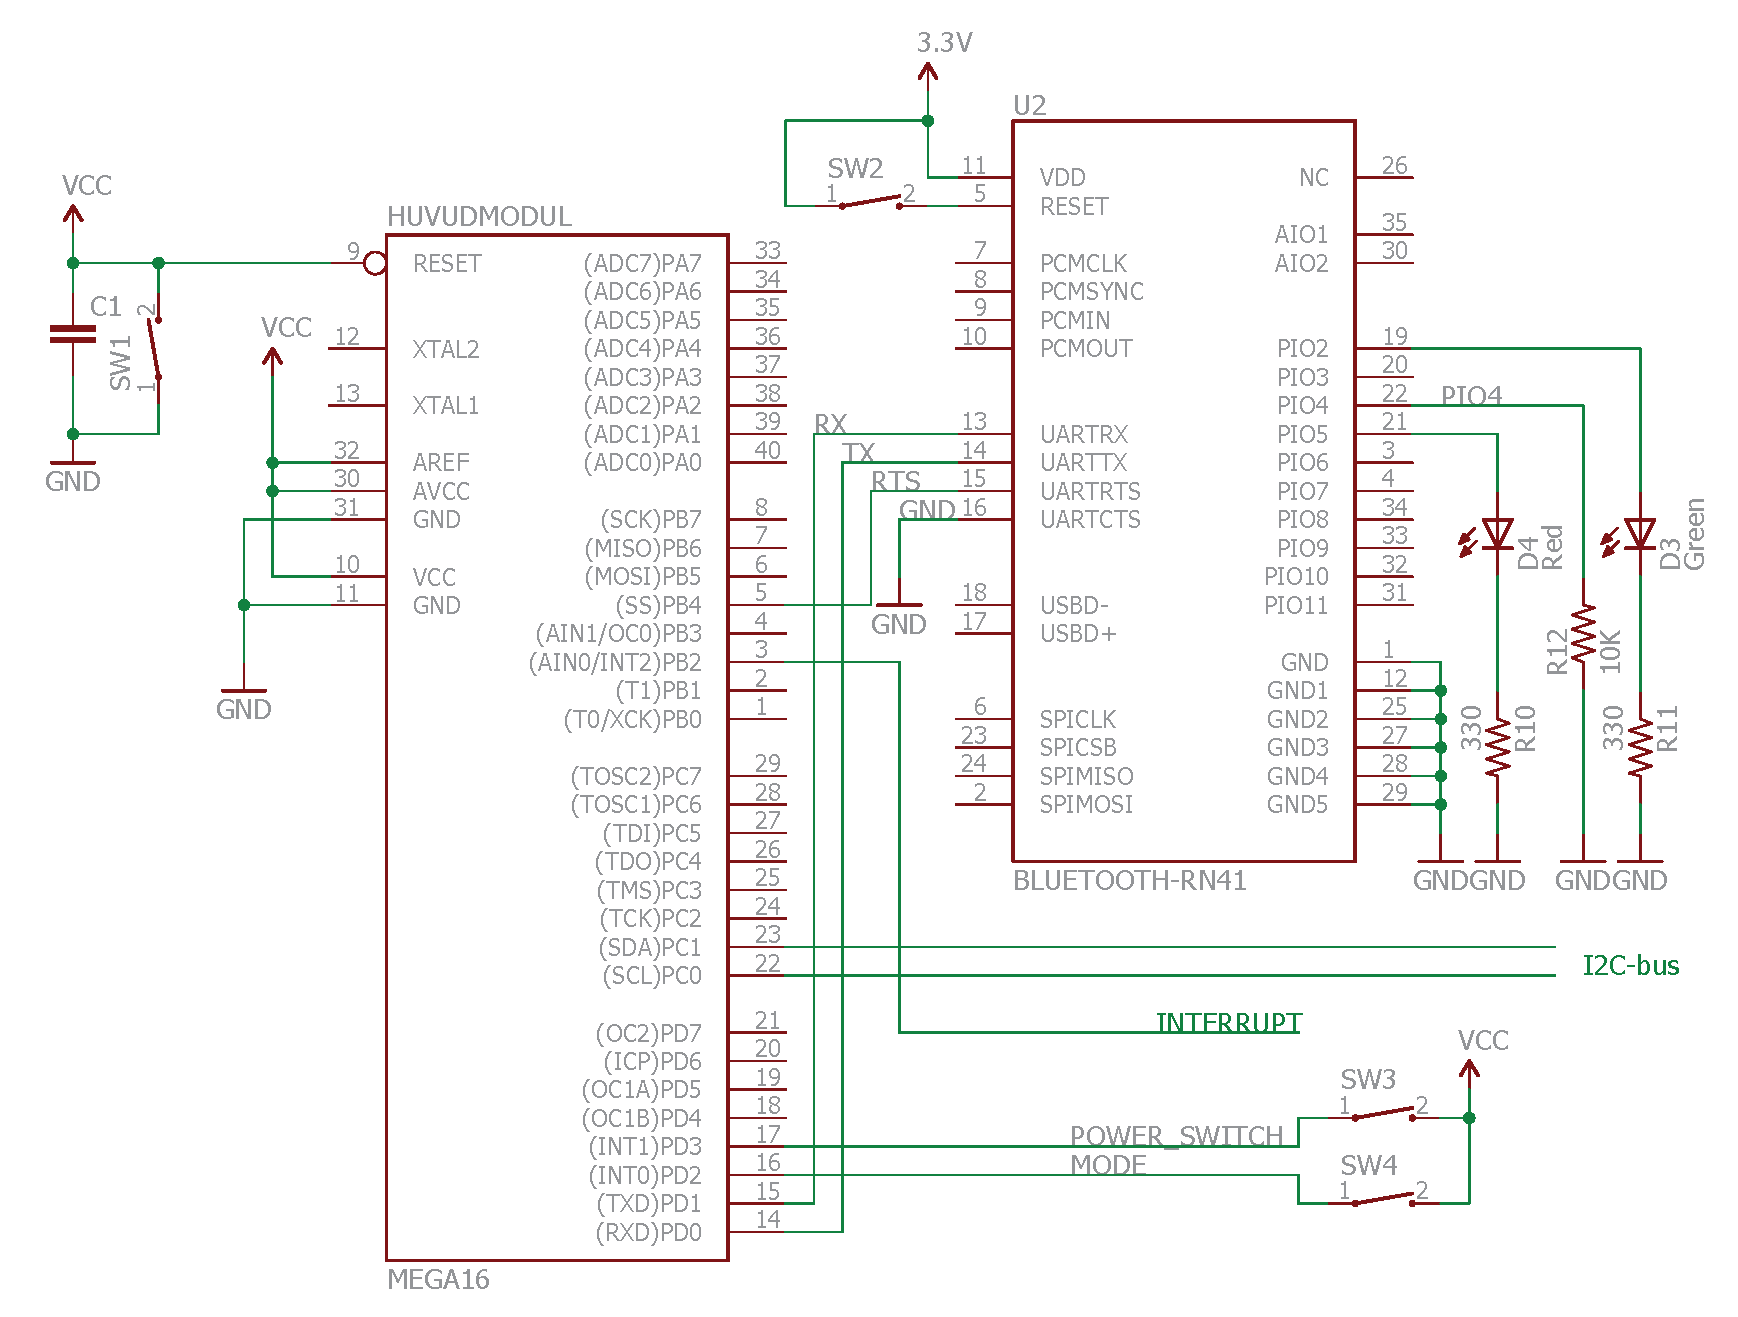
\includegraphics{images/huvudmodul.eps}}
	\caption{Kopplingsschema över huvudmodul \label{kopplingsschema:huvudmodul}}	
\end{figure}

\subsection{Detaljerad beskrivning}

\subsubsection {Körläge}
Knapp för val av körläge kopplas till huvudmodulen på en dataingång. Ingången läses en gång per varv i huvudloopen.

\textbf{\textit{Autonomt läge}}

Kommunikationsflödet i autonomt läge finns beskrivet i figur \ref{autonomousMode}. Beslutet av vilken ny kartmodul, en ruta på ca 40x40 cm\textsuperscript{2}, som roboten ska avsöka tas utifrån den avsökningsalgoritm som implementeras. Oberoende av vilken kartmodul som väljs ser det efterföljande flödet likadant ut. I frågan om när regleringen är klar avvaktas ett avbrott från styrmodulen, vilket beskrivs närmare i avsnitt \ref{styrModul}.

\begin{figure}[htbp]
\centering
\noindent\resizebox{0.9\linewidth}{!}{
	\documentclass[border=10px]{standalone}
\usepackage{tikz}
\usetikzlibrary{patterns}
\usetikzlibrary{shapes.geometric}
\usetikzlibrary{shapes.arrows}
\usepackage{amssymb}
\usetikzlibrary{calc}
\usepackage{verbatim}

\pagestyle{empty}
\begin{document}

\tikzstyle{decision} = [diamond, draw,
    text width=5em, text badly centered, node distance=3cm, inner sep=0pt]
    
\tikzstyle{block} = [rectangle, draw,
    text width=7em, text centered, rounded corners, minimum height=4em]
	
\begin{tikzpicture}[scale=1]

%http://www.texample.net/tikz/examples/simple-flow-chart/

\node[block](start){Start};
\node[block, below of = start, node distance = 3cm](nyModul){Välj ny modul att utforska};
\node[block, right of = nyModul, node distance = 5cm](styrning){Skicka styrkommando till styrmodulen};
%\node[block, right of = styrning, node distance = 4.5cm](sensor){Meddela sensormodulen vilken sensordata som önskas till regleringen};
\node[decision, aspect=1.5,right of = styrning, node distance = 4.5cm](regleringKlar){Är regleringen klar?};
\node[block, right of=regleringKlar, node distance = 4.5cm] (sensorData) {Skicka sensordata till styrmodul};

\draw[->](start) -- (nyModul);
\draw[->](nyModul.east) -- (styrning);
\draw[->](styrning) -- (regleringKlar);
%\draw[->](sensor) -- (regleringKlar);
\draw[->](regleringKlar.east) -- node[above]{nej} (sensorData);
\draw[->](sensorData.north) -| ++(0,1.5) node(lowerright){} -| (regleringKlar.north);
\draw[->](regleringKlar.south) -| ++(0,-1.5) node[above right]{ja} -| (nyModul.south);

	\end{tikzpicture}
	
\end{document}
}
	\cprotect\caption{Flödesschema som beskriver förloppet vid autonom styrning \label{autonomousMode}}	
\end{figure}

\textbf{\textit{Manuellt läge}}

I figur \ref{manualMode} syns kommunikationsflödet när roboten är inställd på manuell styrning.

\begin{figure}[htbp]
\centering
\noindent\resizebox{0.9\linewidth}{!}{
	\documentclass[border=10px]{standalone}
\usepackage{tikz}
\usetikzlibrary{patterns}
\usetikzlibrary{shapes.geometric}
\usetikzlibrary{shapes.arrows}
\usepackage{amssymb}
\usetikzlibrary{calc}
\usepackage{verbatim}

\pagestyle{empty}
\begin{document}

\tikzstyle{decision} = [diamond, draw,
    text width=4em, text badly centered, node distance=3cm, inner sep=0pt]
    
\tikzstyle{block} = [rectangle, draw,
    text width=5em, text centered, rounded corners, minimum height=4em]
	
\begin{tikzpicture}[scale=1]

%http://www.texample.net/tikz/examples/simple-flow-chart/

\node[block](start){Start};
%\node[decision, aspect=2, text width = 8em, below of = start, node distance = 3cm](kommando){Matar användare in styrkommando på tangentbordet?};
\node[block, below of = start, node distance = 3cm, text width = 7em](blåtand){Styrkommando från datormodulen tas emot};
\node[block, right of = blåtand, node distance = 3.5cm, text width = 7em](toStart){Styrkommando skickas från huvudmodul till styrmodul};
\node[decision, aspect=2, text width = 5em, right of = toStart, node distance = 4.5cm](isDone){Har knappen släppts upp?};
\node[block, below of = isDone,node distance = 8em](stop){Skicka stoppsignal till styrmodulen};

\draw[->](start) --  (blåtand);
\draw[->](blåtand) -- (toStart);
\draw[->](toStart) -- (isDone);
\draw[->](isDone) -- node[near start, right]{ja}(stop);
\draw[->](isDone.east) -| node[near start, below]{nej} ++(0.7,2) -| (isDone.north);

	\end{tikzpicture}
	
\end{document}}
	\cprotect\caption{Flödesschema som beskriver förloppet vid manuell styrning \label{manualMode}}	
\end{figure}

\subsubsection {Strömbrytare}
Strömbrytare i form av en knapp som kopplas till en dataingång. Detta medför att förändring inte nödvändigtvis sker på en gång. I figur \ref{strombrytare} visas förloppet då huvudprogrammet är redo att läsa av ingången. 

\begin{figure}[htbp]
\centering
\noindent\resizebox{.6\linewidth}{!}{
	\documentclass[border=10px]{standalone}
\usepackage{tikz}
\usetikzlibrary{patterns}
\usetikzlibrary{shapes.geometric}
\usetikzlibrary{shapes.arrows}
\usepackage{amssymb}
\usetikzlibrary{calc}
\usepackage{verbatim}

\pagestyle{empty}
\begin{document}

\tikzstyle{decision} = [diamond, draw,
    text width=4em, text badly centered, node distance=3cm, inner sep=0pt]
    
\tikzstyle{block} = [rectangle, draw,
    text width=5em, text centered, rounded corners, minimum height=4em]
	
\begin{tikzpicture}[scale=1]

%http://www.texample.net/tikz/examples/simple-flow-chart/

\node[block](start){Start};
\node[block, right of = start, node distance = 2.5cm](mode){Läs av dataingången};
\node[decision, right of = mode](byta){Behöver läge bytas?};
\node[block, right of = byta, node distance = 3.5cm](to_active){Byt läge};
\node[block, below of = byta, node distance = 3cm](to_sleepmode){Behåll nuvarande läge};

\draw[->](start) -- (mode);
\draw[->](mode) -- (byta);
\draw[->](byta) -- node[above]{ja}(to_active);
\draw[->](byta) -- node[right]{nej}(to_sleepmode);


	\end{tikzpicture}
	
\end{document}
}
	\cprotect\caption{Flödesschema som beskriver förloppet vid då strömbrytaren aktiveras \label{strombrytare}}	
\end{figure}

\subsubsection {Sensormodul} 
Sensormodulen är kopplad till huvudmodulens avbrottsingång \verb+INT1+. Händelseförloppet vid aktiverat avbrott kan ses i flödesschemat i figur \ref{avbrott_sensormodul}.

\begin{figure}[htbp]
\centering
\noindent\resizebox{1\linewidth}{!}{
	\documentclass[border=10px]{standalone}
\usepackage{tikz}
\usetikzlibrary{patterns}
\usetikzlibrary{shapes.geometric}
\usetikzlibrary{shapes.arrows}
\usepackage{amssymb}
\usetikzlibrary{calc}
\usepackage{verbatim}

\pagestyle{empty}
\begin{document}

\tikzstyle{decision} = [diamond, draw,
    text width=4em, text badly centered, node distance=3cm, inner sep=0pt]
    
\tikzstyle{block} = [rectangle, draw,
    text width=5em, text centered, rounded corners, minimum height=4em]
	
\begin{tikzpicture}[scale=1]

%http://www.texample.net/tikz/examples/simple-flow-chart/

\node[block](start){Start};
\node[decision, below of = start](int2){Positiv flank på \verb+INT1+?};
\node[block, right of = int2, node distance = 3cm](in_sensor){Initiera kommunkation med sensormodul};
\node[block, right of = in_sensor, node distance = 3cm](data_sensor){Ta emot data från sensormodul};
\node[block, right of = data_sensor, node distance = 3cm](in_styr){Initiera kommunikation med styrmodul};
\node[block, right of = in_styr, node distance = 3cm](data_styr){Skicka data till styrmodul};
\node[block, right of = data_styr, node distance = 3cm](in_pc){Initiera kommunikation med datormodul};
\node[block, right of = in_pc, node distance = 3cm](data_pc){Skicka data till datormodul};

\draw[->](start) -- (int2);
\draw[->](int2) |- node[near start,right]{nej} ++(-1.5,-1.5) |- (int2);
\draw[->](int2) -- node[above]{ja} (in_sensor);
\draw[->](in_sensor) -- (data_sensor);
\draw[->](data_sensor) -- (in_styr);
\draw[->](in_styr) -- (data_styr);
\draw[->](data_styr) -- (in_pc);
\draw[->](in_pc) -- (data_pc);

	\end{tikzpicture}
	
\end{document}
}
	\cprotect\caption{Flödesschema som beskriver förloppet vid avbrott på ingång \verb+INT1+ \label{avbrott_sensormodul}}	
\end{figure}

\subsubsection{Styrmodul}
\label{styrModul}
Styrmodulen är kopplad till huvudmodulens avbrottsingång  \verb+INT0+. En avbrottssignal triggas på positiv flank och skickas när regleringen av nuvarande styrkommando är klart. Huvudmodulen kan då ta ett nytt beslut enligt flödesschemat i figur \ref{autonomousMode}.

\subsubsection{Kartläggning}
Eftersom kartan enligt appendix C består av moduler på 40x40cm, räcker det att uppdatera kartläggningen en gång per sådan modul. Genom mätvärden från lasersensor, då den riktas framåt, kan avståndet till den främre väggen beräknas. Denna signal samplas ofta nog så att roboten kan beräkna när den har färdats till nästa modul. 

IR-sensorerna på robotens sida kan agera i avståndsområdet 5-30 cm och bottnas med andra ord när en sväng eller korsning upptäcks. Utifrån denna information kopplar kartläggningen ihop föregående modul med den typ av korsning som roboten står i. 

Kartläggningsalgoritmen är av väggföljartyp. Eftersom banan är uppbyggd så att varken höger- eller vänsterföljning prioriteras, se appendix C, så faller valet på högerföljning. Med andra ord följer roboten höger vägg och försöker först att svänga höger, därefter köra rakt fram och svänger vänster allra sist. Eftersom roboten endast ska finna den kortaste vägen från ingången till nödställde behöver nödvändigtvis inte hela kartan utforskas. Exempelvis, ifall fågelvägen från roboten till ingången är längre än en redan utforskad rutt ska roboten inte fortsätta utforska den korridoren.

Mjukvarumässigt representeras kartan med hjälp av noder och bågar, se figur \ref{labToGraph} för ett exempel av labyrintkonvertering. En ny nod bildas vid varje korsning eller där roboten tvingas svänga. Bågkostnaden utgör det relativa avståndet mellan de två kopplade noderna där det relativa avståndet mellan två moduler är en enhet.

\begin{figure}[htbp]
\centering
\noindent\resizebox{.6\linewidth}{!}{
	\documentclass[border=10px]{standalone}
\usepackage{tikz}
\usetikzlibrary{patterns}
\usetikzlibrary{shapes.arrows}
\usepackage{amssymb}
\usetikzlibrary{calc}
\usetikzlibrary{positioning}
\usepackage{verbatim}
\begin{document}
	
\begin{tikzpicture}[scale=1]
		
		\draw[thick, ,draw=none, pattern=north west lines, pattern color=green] (1,3) rectangle (2,4);
		\draw[thick] (0,0) -- (0,5) -- (5,5) -- (5,0) -- (1,0);
		\draw[thick] (4,0) -- (4,4);
		\draw[thick] (4,1) -- (1,1);
		\draw[thick] (1,2) -- (3,2) -- (3,3) -- (1,3) -- (1,4) -- (3,4);
		
		\draw[thick, ->] (.5,-.5) -- (.5,0);
		
		\node[] at (6.5,2.5) {\huge $\Leftrightarrow$};
		
		\tikzset{every node/.style={minimum size=.5cm, align=center,anchor=center, on grid,x=1.5cm,y=1.5cm}}
		\node[draw=black, circle] 							(A) at (5.5,-.3) {};
		\node[above=1 of A, draw=black, circle] 				(B) {};
		\node[above=1 of B, draw=black, circle] 				(C) {};
		\node[above=2 of C, draw=black, circle] 				(D) {};
		\node[right=3 of D, draw=black, circle] 				(E) {};
		\node[right=1 of E, draw=black, circle] 				(F) {};
		\node[below=4 of F, draw=black, circle] 				(G) {};
		\node[below=1 of E, draw=black, circle] 				(H) {};
		\node[left=2 of H, draw=black,fill=green, circle] 	(I) {};
		\node[below=2 of H, draw=black, circle] 				(J) {};
		\node[right=2 of C, draw=black, circle] 				(K) {};
		\node[right=3 of A, draw=black, circle] 				(L) {};
		
		\draw[thick,draw=green] (A) -- node[left] 	{1} (B) ;
		\draw[thick] 			(B) -- node[left] 	{1} (C);
		\draw[thick] 			(C) -- node[left] 	{2} (D);
		\draw[thick] 			(D) -- node[above] 	{3} (E);
		\draw[thick] 			(E) -- node[above] 	{1} (F);
		\draw[thick] 			(F) -- node[right] 	{4} (G);
		\draw[thick] 			(E) -- node[right] 	{1} (H);
		\draw[thick,draw=green] (H) -- node[above] 	{2} (I);
		\draw[thick,draw=green] (H) -- node[right] 	{2} (J);
		\draw[thick,draw=green] (J) -- node[above] 	{3} (B);
		\draw[thick] 			(A) -- node[above] 	{3} (L);
		\draw[thick] 			(C) -- node[above] 	{2} (K);
		
	\end{tikzpicture}
\end{document}}
	\caption{En labyrint och dess motsvarande nätverk. Bågkostnaderna är det relativa avståndet och den optimala vägen är markerad grön.\label{labToGraph}}	
\end{figure}

När kartan är representerad som ett nätverk och roboten med säkerhet har utforskat den kortaste vägen mellan ingång och nödställd, påbörjas optimeringen. Optimeringen för att hitta den kortaste vägen sker med hjälp av optimerande metoder för att lösa minkostnadsnätverk.

Roboten tillämpar optimeringsmodellen A* vilken är en vidareutveckling av Dijkstras algoritm. A* är en bäst-först algoritm med målet att finna den billigaste vägen mellan två noder. I grund och botten finns samma maskineri som i Dijkstras algoritm fast där noder avsöks i stigande ordning av
\begin{equation*}
	f(n) = g(n) + h(n)
\end{equation*}
där $g(n)$ utgör kostnaden av rutten från startnod till nod $n$ och $h(n)$ en heuristik som estimerar den billigaste vägen från nod $n$ till slutnod. Med andra ord är Dijkstras algoritm ett speciallfall av A* där $h(n) = 0$. Heuristiken som används är det så kallade \emph{Manhattan}-avståndet eftersom labyrintens korsningar är ortogonala.

Låt $V$ vara mängden av samtliga noder, $S$ mängden av avsökta noder och $Q$ mängden av oavsökta noder. Då implementeras algoritmens utifrån pseudokoden i algoritm \ref{astar}.

\begin{algorithm}[H]
	\caption{A*} \label{astar}
	\begin{algorithmic}[1]
		\Function{AStarAlgorithm}{Graph, s}	
			\State $g(s) \gets 0$
			\State $f(s) \gets g(s) + h(s)$
			\ForAll {$v\in V - \{ s\}$}
				\State $g(v) \gets \infty$
				\State $f(v) \gets \infty$
			\EndFor
			
			\State $S \gets \emptyset$
			\State $Q \gets V$
			
			\While {$Q \neq \emptyset$}
				\State $u \gets \textrm{minFvalue}(Q,f)$%
				\Comment{Välj nod med lägst $f(n)$}
				\State $S \gets S +  \{ u\}$
				\State $Q \gets Q - \{ u\}$
				\ForAll {$v \in \textrm{neighbours}(u)$}
				\Comment{Itererare över grannar till $u$}
					\If {$g(u) + w(u,v) < g(v)$}
						\State $g(v) \gets g(u) + w(u,v)$
						\State $f(v) \gets g(v) + h(v)$
					\EndIf
				\EndFor
			\EndWhile
			
			\Return $g$
		\EndFunction
	\end{algorithmic}
\end{algorithm}
  

\subsection{Hårdvara}
Huvudmodulen kommer kräva följande hårdvara:
\begin{itemize}
	\item ATmega16
	\item  Bluetooth\textsuperscript{\circledR}  (Firefly)
\end{itemize}


\subsection{Mjukvara}
Koden i huvudmodulen är skriven i C. 

\pagebreak
\section{Delmodul 2 - Sensormodul}
Sensormodulens uppdrag är att kommunicera med både sensorerna och huvudmodulen. Mätdata samplas med konstant frekvens och konverteras därefter till motsvarande SI-enhet. För avståndssensorerna innebär detta att den analoga inspänningen konverteras till ett digitalt värde i enheten meter.

Den främre avståndssensorn (laser-sensorn) placeras på ett roterande servo så att den kan \emph{scanna} korridoren roboten befinner sig i. Detta förutsätter att servot går att styra så att vinkelutslaget går att beräkna med godtycklig precision. Tillåter inte servot en sådan styrning placeras laser-sensorn så att den konstant pekar rakt framåt.

Vinkelhastighets-sensorerna används för att beräkna vinkelutslag då roboten tar en sväng. Mätdatan behöver därför integreras under ett tidsintervall och konverteras till en vinkel. Hur den nödställde ska representeras är ännu inte fastställt. Förslagsvis används en IR-fyr i kombination med en IR-sensor. Sensormodulens uppdrag blir då att ta beslutet om när den nödställde är funnen.

\begin{figure}[htbp]
\centering
\noindent\resizebox{\linewidth}{!}{
	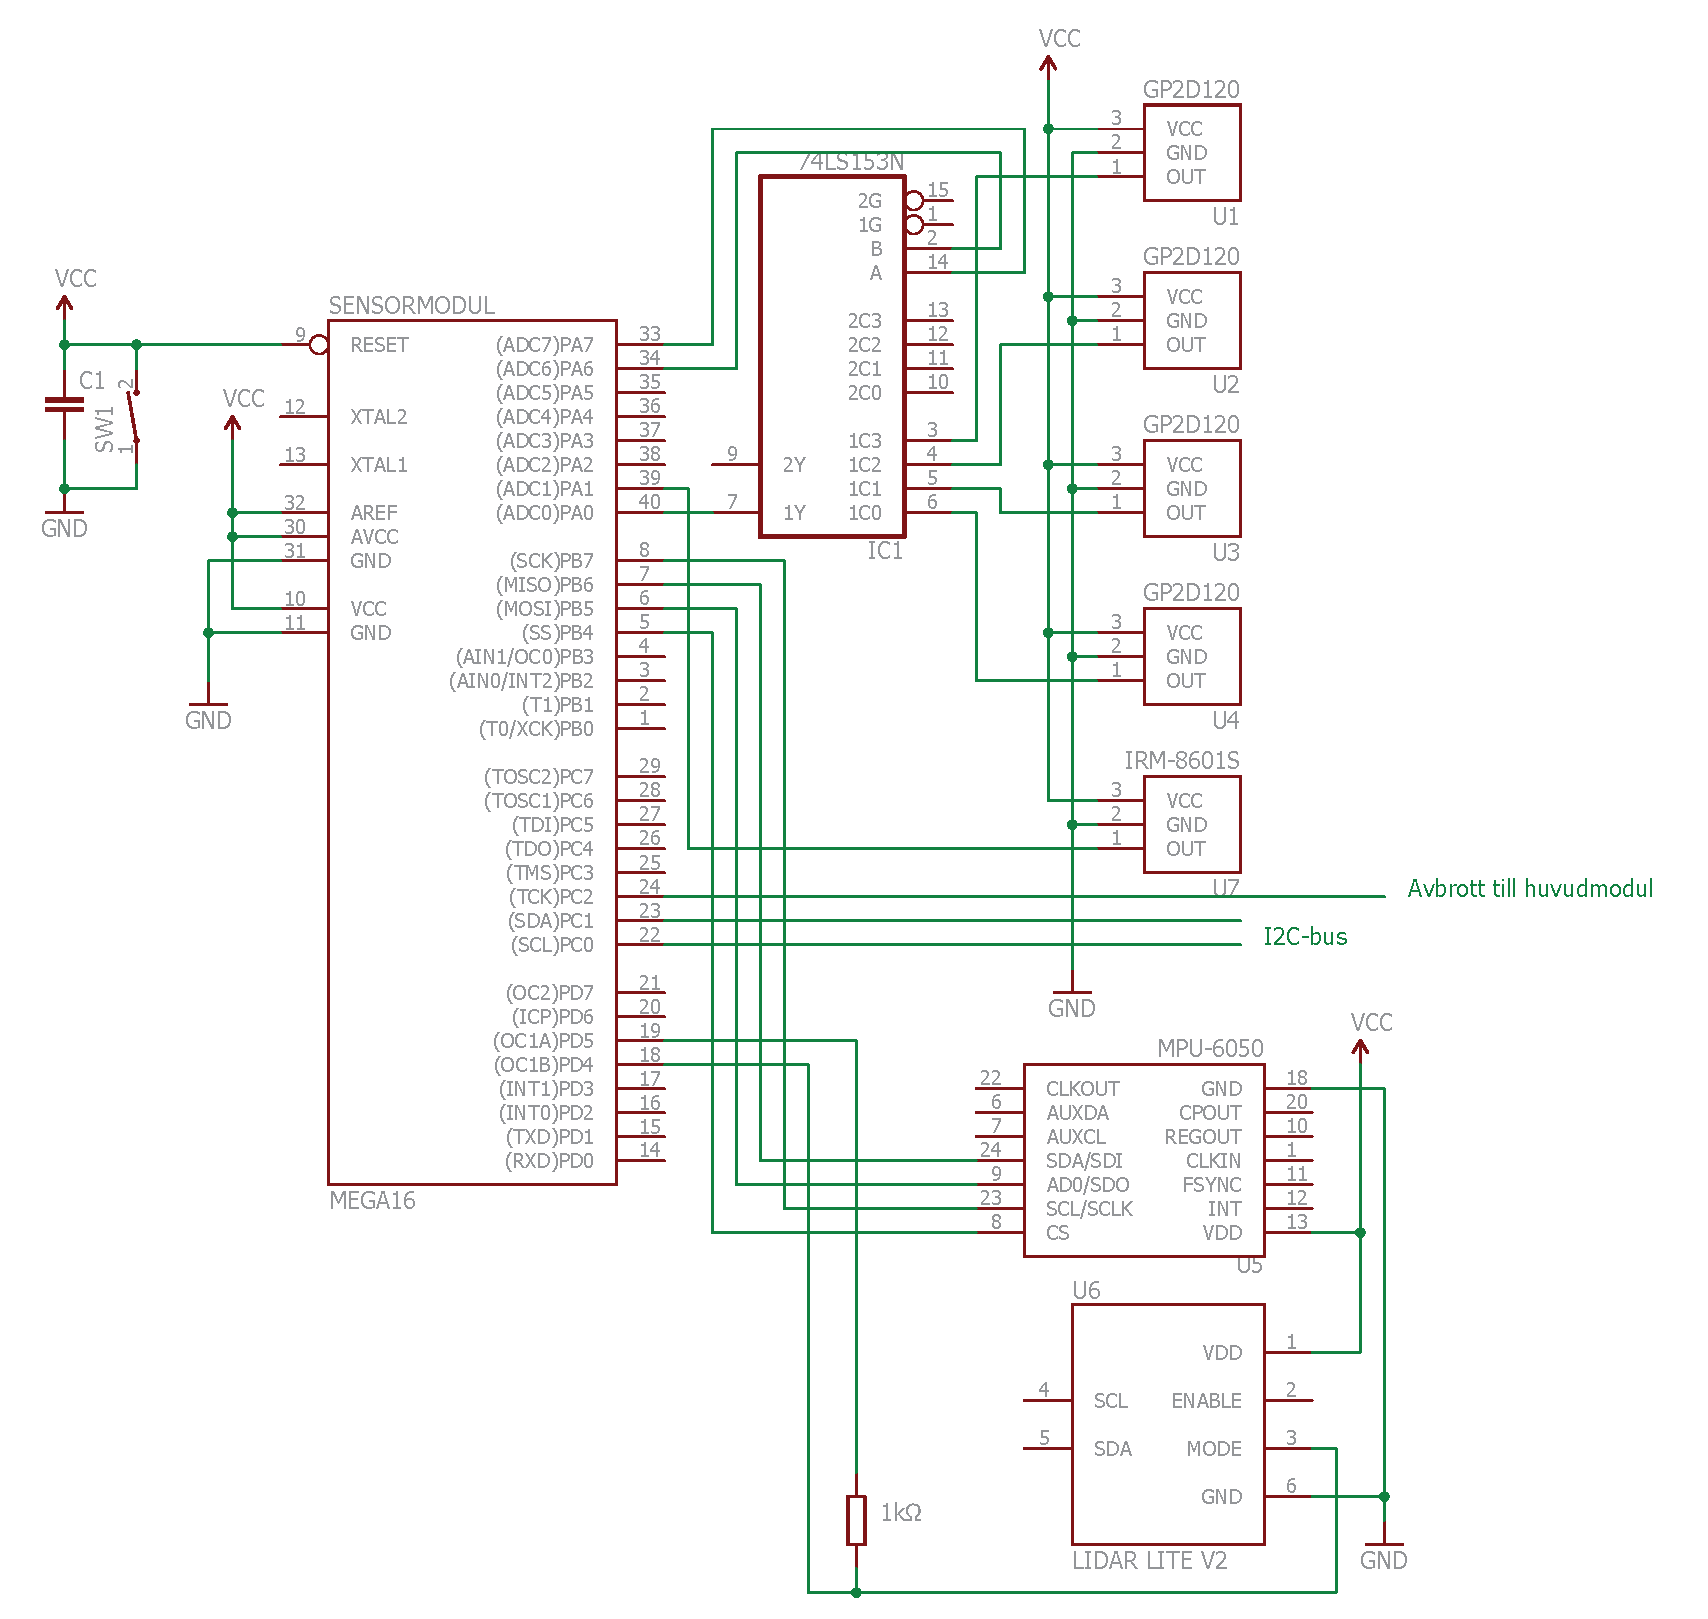
\includegraphics{images/sensormodul.eps}}
	\caption{Kopplingsschema över sensormodul \label{kopplingsschema:sensormodul}}	
\end{figure}
 
\subsection{Hårdvara}
Den hårdvara som sensormodulen kommer att kräva är:

\begin{itemize}
\item{Processorenhet, ATmega16 x 1}
\item{IR-sensor, GP2D120 x 2}
\item{Laser-sensor, LIDAR-Lite v2 x1}
\item{Gyro/accelerometer, MPU-6500 x 1}
\item{IR-detektor, IRM-8601-S x 1}

\end{itemize}

\subsection{Detaljerad beskrivning}

Sensormodulens processorenhet, \verb+ATmega16+, är ansluten med en I\textsuperscript{2}C-buss. Den har som uppgift att kommunicera med huvudmodulen, där sensormodulens processorenheter agerar som slavenhet i förhållande till huvudmodulens dito. 
%Den andra I\textsuperscript{2}C-bussen kommunicerar med Lasersensorn, LIDAR-Lite v2, samt gyro/accelerometern, MPU-6500. I fallet med den senare databussen så agerar sensormodulens processorenhet som masterenhet i förhållandet med lasersensorn och gyro/accelerometern.
IR-sensorn GP2D120 och IR-detektorn IRM-8601-S ansluts direkt till processorenhetens ingångar för AD-omvandling. Figur \ref{kopplingsschema:sensormodul} visar en övergripande bild över sensormodulens implementation med dess respektive delkomponenter. 

\subsubsection{Processorenhet, ATmega16}
Insamlat sensordata bearbetas i modulens processorenhet för att därefter kommuniceras till huvudmodulen. Figur \ref{kopplingsschema:sensormodul} illustrerar \verb+ATmega16+ och dess ingångar, samt hur respektive sensorenhet ska kopplas samman med processorn. 

\subsubsection{Laser-sensor, LIDAR-Lite v2}
Lidar-Lite v2 är en kraftfull lasersensor av begränsad storlek med ett flertal funktioner ändamålsenliga för exempelvis en undsättningsrobot. Utöver att kunna möta avstånd, så kan den dessutom mäta hastighet och signalstyrka hos mål på upptill 40 meters avstånd. Detta med en felmarginal på 0,025 meter. Andra fördelar hos sensorn inkluderar låg strömkonsumtion och en upplösning 0,01 meter \cite{7131685}.

%Kommunikationen mellan Lidar-Lite v2 och processorenheten, \verb+Atmega16+, kommer att ske via ett I\textsuperscript{2}C-interface som lasersensorn kommer med i sitt grundutförande. Figur [??] konkretiserar hur implementationen av databussen ska genomföras. 

\subsubsection{IR-sensor, GP2D120}
För att kunna reglera på ett önskat sätt behöver roboten veta hur den förhåller sig i förhållande till sidoväggarna. Eftersom roboten ska kunna köra i mitten av korridorer med ca 40 centimeters bredd, och roboten själv är ca 20 cm bred, kommer ett avstånd mellan sidoväggarna och roboten på 10 cm vara önskvärt. För detta är IR-sensorn GP2D120 bra, eftersom den kan mäta avstånd till objekt som befinner sig på 4-30 cm ifrån sensorn. 

Mätningen av avstånd sker genom att IR-ljus med en viss våglängd skickas ut från sensorn, reflekteras mot väggarna för att till sedan sensorns detektorer känner av det reflekterade ljuset. Genom att mäta den vinkel reflektionen sker med kan avståndet till väggen bedömas. GP2D120 är relativt enkel och har enbart två ingångar som ska kopplas till en 5 volts strömkälla, respektive en jord.  Utsignalen är analog i form av ström, där IR-sensorerna behöver lågpassfiltreras.
%Om robotens reglering inte är tillräckligt bra är det risk att avståndssensorn tappar precision, %eller till och med mister avståndsbedömning helt. Det beror på att om roboten inte kör %parallellt med väggen kommer det utstrålade ljuset att reflekteras med en för stor vinkel för %att detektorerna ska kunna uppfatta reflektionen.

\subsubsection{Gyro/accelerometer, MPU-6050}
%\item[Vinkelhastighet] \hfill \\
I den labyrint där roboten ska hitta den nödställde kommer det finnas korsningar, vilket ställer krav på roboten att svänga. För att klara av detta används MPU6050, som får roboten att rotera. Genom att mäta hur mycket roboten roterar kan den avgöra när en 90-graderssväng är genomförd och det är dags att sluta rotera. Hastigheten på rotationen kan ställas in efter önskat behov.



% och informationen från sensorn kommer att förmedlas via ett I\textsuperscript{2}C-buss-interface.
 
\subsubsection{IR-detektor, IRM-8601-S}
IR-detektorn IRM-8601-S används i syfte att identifiera den nödställde, vilken ska sända ut en IR-signal. Liksom figur \ref{kopplingsschema:sensormodul} illustrerar så är IRM-8601-s förhållandevis trivial i sitt utförande, enheten har 2 ingångar vilka ska anslutas med 5 V samt jord. 

Liksom i fallet med GP2D120 så är IR-dektorns utsignal analog, vilket innebär att signal bör AD-omvandlas.  Omvandlingen sker via 

\begin{equation*}
	\textrm{Digitalt värde} = \frac{255}{5}V_{out}
\end{equation*}

där den maximala utsignalen är 5 volt. Det analoga värdet delas upp i 256 digitala värden som motsvarar olika spänningar. Sambandet mellan spänning och avstånd till väggen kan utläsas av figur \ref{IR_avstand}.

\begin{figure}[htbp]
	\centering
	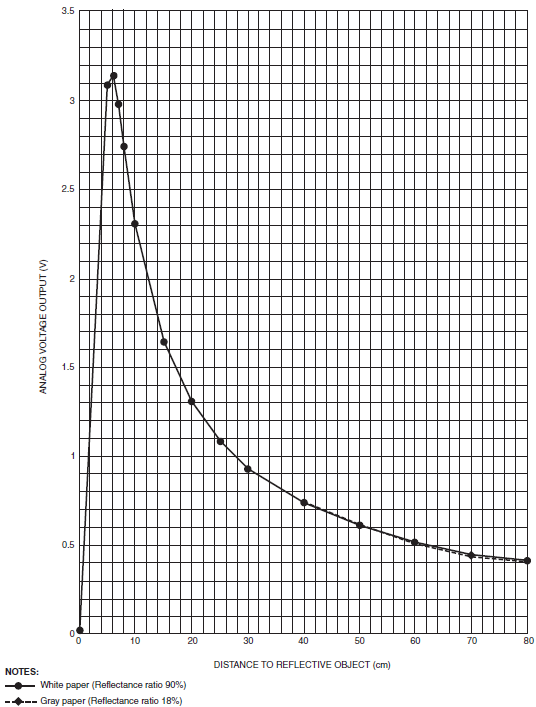
\includegraphics[scale=0.4]{images/IR_avstand}
	\caption{Förhållande mellan analog spänning och avstånd \label{IR_avstand}}
\end{figure}
%\item[Identifierare av nödställd] \hfill \\


\subsection{Mjukvara}
Sensormodulens kod är skriven i C och har som huvuduppgift att göra om de analoga signaler som uppmäts till digitala signaler som skickas visare till huvudmodulen. De olika sensorerna tar in olika typer av analoga signaler, vilket innebär att även fler typer av omvandlingar behöver vara möjliga. Alla omvandlingar sker i enhetens processorenhet, \verb+ATmega16+. 

\subsubsection{IR-sensorerna}
GP2120 och IRM-8601-S reflekterar ljus för att identifiera nödställd och mäta avstånd och vinklar mot omgivande objekt. Utsignalen vid dessa operationer är spänning (Vout), vilket behöver göras om till ett digitalt värde för att kunna skicka vidare informationen. 


\begin{figure}[htbp]
\centering
\noindent\resizebox{.5\linewidth}{!}{
	\documentclass[border=10px]{standalone}
\usepackage{tikz}
\usetikzlibrary{patterns}
\usetikzlibrary{shapes.geometric}
\usetikzlibrary{shapes.arrows}
\usepackage{amssymb}
\usetikzlibrary{calc}
\usepackage{verbatim}

\pagestyle{empty}
\begin{document}

\tikzstyle{decision} = [diamond, draw,
    text width=4em, text badly centered, node distance=3cm, inner sep=0pt]
    
\tikzstyle{block} = [rectangle, draw,
    text width=5em, text centered, rounded corners, minimum height=4em]
	
\begin{tikzpicture}[scale=1]

%http://www.texample.net/tikz/examples/simple-flow-chart/

\node[block](start){Start};
\node[decision, below of = start](int2){ADIF};
\node[block, right of = int2, node distance = 3cm](in_sensor){Omvandlar avstånd till lämplig SI-enhet};
\node[block, right of = in_sensor, node distance = 3cm](data_sensor){Lägger omvandlat data på separat dataregister};
%\node[block, right of = data_sensor, node distance = 3cm](in_styr){Initiera kommunikation med styrmodul};
%\node[block, right of = in_styr, node distance = 3cm](data_styr){Skicka data till styrmodul};
%\node[block, right of = data_styr, node distance = 3cm](in_pc){Initiera kommunikation med datormodul};
%\node[block, right of = in_pc, node distance = 3cm](data_pc){Skicka data till datormodul};

\draw[->](start) -- (int2);
\draw[->](int2) |- ($(int2.south west) + (-0.7,-0.6)$) |- node[near start,left]{nej}(int2);
\draw[->](int2) -- node[above]{ja} (in_sensor);
\draw[->](in_sensor) -- (data_sensor);
%\draw[->](data_sensor) -- (in_styr);
%\draw[->](in_styr) -- (data_styr);
%\draw[->](data_styr) -- (in_pc);
%\draw[->](in_pc) -- (data_pc);

	\end{tikzpicture}
	
\end{document}
}
	\caption{Flödesschema för hur AD-omvandling ska initieras\label{datormodul:Avbrott_ADC}}	
\end{figure}


\FloatBarrier
\subsubsection{LIDAR-Lite}
Lasersensorn LIDAR-Lite används för att scanna av omgivningen och ge bild av miljön roboten rör sig i. Den kommer liksom IR-sensorerna få ut en analog utsignal i volt, som behöver konverteras till ett digitalt värde innan det skickas till huvudmodulen. Även här kommer tester få göras för att hitta sambandet mellan avstånd och spänning.

\subsubsection{MPU-6050}
Rotationen av roboten genomförs av MPU-6050 som får roboten att rotera önskat antal grader. För att lyckas rotera lagom mycket behöver tester genomföras för att uppmäta hur snabbt (grader per sekund) roboten roterar. Utifrån utmätt data kan en omvandlingstabell skapas.

\pagebreak
\section{Delmodul 3 - Styrmodul}
Styrmodulens uppgift är att översätta styrkommandon till servostyrning av de fyra hjulen och gripklon. Styrkommandona kommer via I\textsuperscript{2}C-bussen från huvudmodulen och konverteras därefter till en PWM-sekvens. PWM-sekvensen skickas till gripklon respektive H-bryggorna som styr ett hjulpar var. 

Kopplingsschemat ser ut enligt figur \ref{kopplingsschema:styrmodul}, det framgår från figuren att utgångarna från \verb+ATmega16+ räcker för modulens ändamål. Både avbrottsingång \verb+INT0+ och \verb+INT1+ används inte men reservas ifall ytterligare funktionalitet önskas lägga till. Det finns även möjlighet att att styra en extra komponent via PWM eftersom utgången \verb+OC2+ är oanvänd.  

Prestandan hos \verb+ATmega+16 räcker för modulens syfte. 

\begin{figure}[htbp]
\centering
\noindent\resizebox{\linewidth}{!}{
	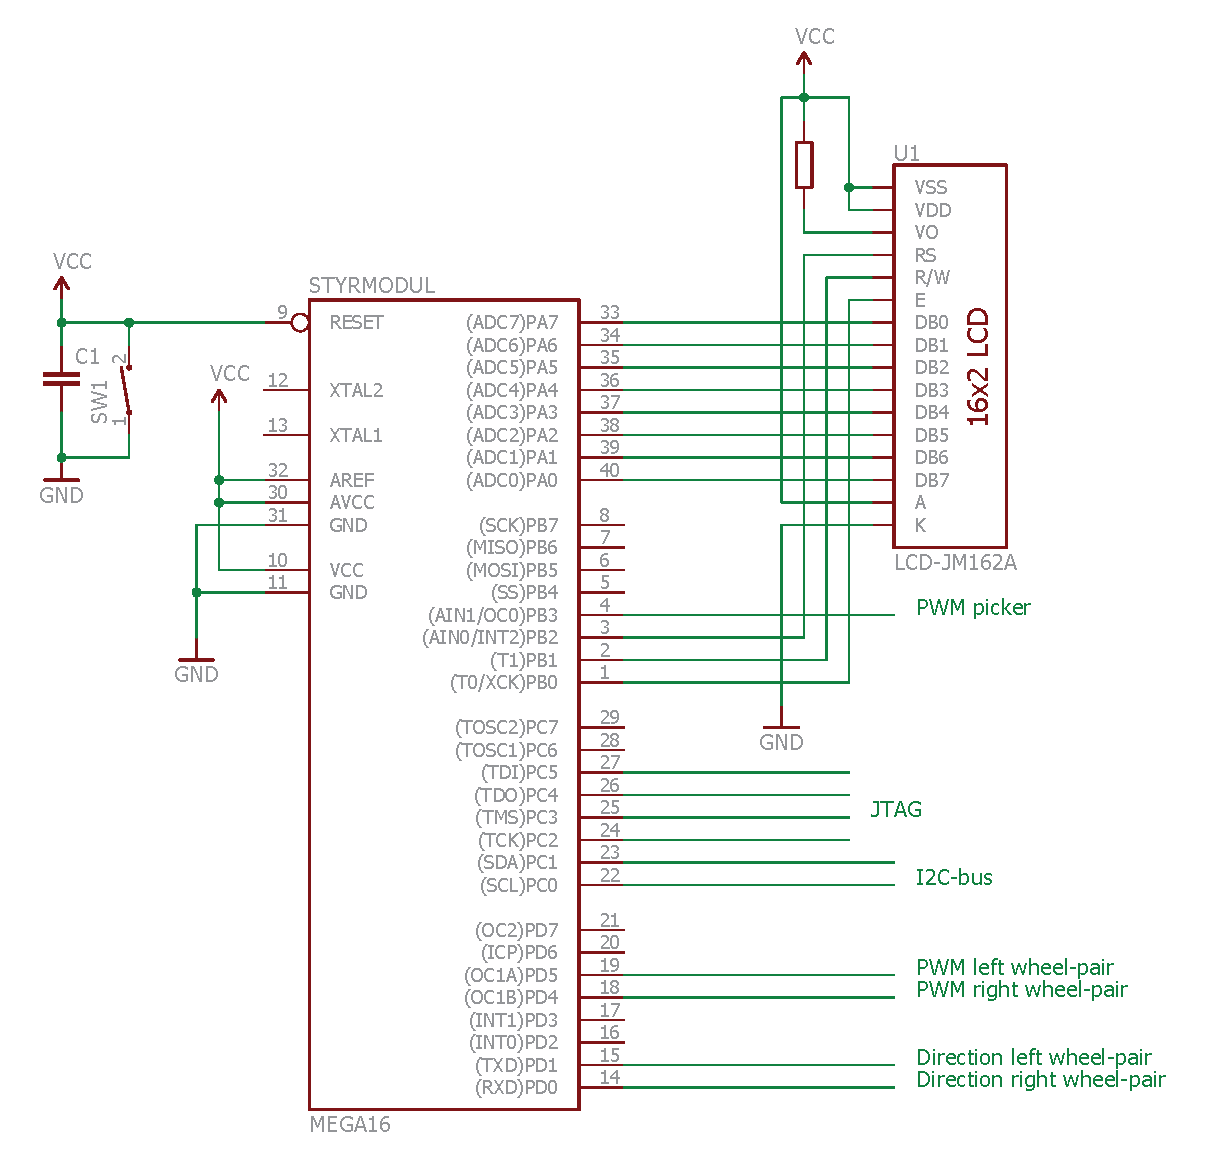
\includegraphics{images/styrmodul.eps}}
	\caption{Kopplingsschema över styrmodul \label{kopplingsschema:styrmodul}}	
\end{figure}
 
\subsection{Detaljerad beskrivning}
Nedan följer en beskrivning av vilka styrkommandon styrmodulen ska kunna ta emot, hur kommunikationsprotokollet ser ut, hur regleringen ska ske samt lite övrig fakta kring modulen.

\subsubsection{Styrkommandon}\label{Styrkommandon}
Styrmodulen tar emot kommandon från huvudmodulen och verkställer dessa. Följande kommandon kommer kunna skickas: \textit{reglering av/på, gripklo öppna/stäng, fram/bak, sväng höger/vänster, rotera höger/vänster och stopp}. Kommandot \textit{reglering av/på} ställer in styrmodulen för manuell eller autonom körning, vilket påverkar tolkningen av det data som skickas från huvudmodulen.

Tillsammans med kommandona för rörelse skickas även ett tal som, beroende på om reglering är aktiverad eller inte, anger en sträcka/vinkel för förflyttningen eller med vilken hastighet (i procent av maxhastighet) förflyttningen ska utföras. Ett kommando kan exempelvis se ut såhär: \textit{fram 80}, varpå roboten antingen kör framåt 80 cm eller med 80\% av maxhastighet, beroende på om regleringen är aktiverad eller inte. Modulen kommer vara designad så att ett körkommando gäller tills dess att ett nytt kommando skickas, varför även kommandot för \textit{stopp} är nödvändigt.

Eftersom kommandona till styrmodulen skickas på den form som visats ovan kommer all reglering behöva ske i styrmodulen. Därför kommer även mätdata att tas emot från huvudmodulen. Beroende på vilken typ av förflyttning roboten utför så kommer följande sensorvärden att skickas från huvudmodulen:
\begin{itemize}
	\item fram/bak - avstånd till vägg fram och på sidorna.
	\item sväng höger/vänster - inga (kommandot används enbart vid manuell styrning och behöver således inte regleras).
	\item rotera höger/vänster - vinkel och vinkelhastighet.
\end{itemize}
Dessa sensorvärden kommer skickas med en frekvens av 10-20 Hz förutsatt att reglering är aktiverad, det vill säga vid autonom styrning av roboten.

När styrmodulen har genomfört sitt körkommando från huvudmodulen skickar den en positiv flank på \verb+PB4+. Denna utgång är kopplad till en avbrottsingång på huvudmodulen och tolkas som att styrmodulen är redo för ett nytt kommando. 

\subsubsection{Reglering}
Vid manuell styrning av roboten sker ingen reglering. Detta för att användaren ska få ohämmad kontroll över roboten och förväntas sköta ``regleringen'' manuellt. Vid autonom styrning kommer dock alla förflyttningar behöva regleras. Som nämnt i avsnitt \ref{Styrkommandon} kommer huvudmodulen skicka relevanta sensorvärden vid autonom körning. Beroende på vilket styrkommando som skickats väljer styrmodulen sedan en styrmod och reglerar rörelsen. De olika styrmodulerna och hur deras reglering sker finns beskrivet mer ingående i avsnitt \ref{mjukvarureglering}.

\subsubsection{Övrigt}
Plattformen som roboten byggs på har färdiga kretsar för att styra chassits hjul. Hjulen kan styras parvis (höger och vänster) genom att sätta en bit för att bestämma rotationsriktningen och sedan skicka en PWM-signal för att bestämma rotationshastigheten. Roboten styrs alltså differentiellt, dvs genom olika hastighet på höger och vänster sida.

Roboten ska även vara utrustad med en gripklo, för att kunna greppa de förnödenheter som ska transporteras. Klons aktiva del består av ett servo av typen \verb+RG-180+ som styrs med en PWM-signal.

Det ska även finnas en alphanumerisk LCD-display, av typen \verb+LCD JM162A+, på roboten, som används för att visa relevanta sensorvärden vid reglering. Den har totalt 16 pinnar, varav åtta är databitar, tre används för konfiguration och resterande är referenssignaler och strömtillförsel.

\subsection{Hårdvara}
Styrmodulen kommer kräva följande hårdvara:
\begin{itemize}
	\item ATmega16
	\item Robotplattform (Terminator)
	\item Gripklo %Specificera senare
\end{itemize}

\subsection{Mjukvara}
Koden för styrmodulen är skriven i C och består främst av två delar, reglering och display. Gripklon styrs direkt av ett styrkommando och kan endast öppnas respektive stängas.


\subsubsection{Display}
Displayen är en alphanumerisk 16x2 LCD-display och ska visa utvalda sensorvärden i realtid. I koden används drivrutinen \emph{lcd.h} för att initiera och skriva text till displayen. Genom att anropa initieringsmetoden rensas displayen och pekaren placeras på rätt position. Därefter skrivs typen av mätvärde och det faktiska värdet ut. Tack vare två rader kan flera mätvärden skrivas ut samtidigt, förslagsvis ett i respektive hörn av displayen.

Utskriften till displayen sker i huvudloopen och i takt med att nya mätvärden tas emot.

\subsubsection{Reglering} \label{mjukvarureglering}
\begin{figure}[H] 
\centering
\noindent\resizebox{.8\linewidth}{!}{
	\import{images/}{cartesian}}
	\caption{Väggföljning\label{robotwall}}	
\end{figure}

När styrmodulen tar emot ett kommando från huvudmodulen så regleras servona utifrån de senaste mottagna sensorvärdena. Den reglering som programmeras till modulen består av tre komponenter. Den ena ser till att roboten färdas i mitten av korridoren, den andra anpassar hastigheten utifrån korridorens längd och den tredje ser till att en sväng tas vinkelrätt.

Isak: fortsätt på stycket och förklara regleringen utifrån din förstudie

\pagebreak
\section{Delmodul 4 - Datormodul}
Datormodulens syfte är att presentera ett gränssnitt för att styra, kartlägga och felsöka roboten i realtid. Kommunikationen sker via Bluetooth\textsuperscript{\circledR} och består av styrkommandon (datormodul $\rightarrow$ huvudmodul) samt mätvärden och karta (huvudmodul $\rightarrow$ datormodul). 

\subsection{Detaljerad beskrivning}
Mjukvarans grafiska gränssnitt konstrueras enligt figur \ref{datormodul:software}.

\begin{figure}[htbp]
\centering
\noindent\resizebox{.5\linewidth}{!}{
	\documentclass[border=10px]{standalone}
\usepackage{tikz}
\usetikzlibrary{patterns}
\usetikzlibrary{shapes.arrows}
\usepackage{amssymb}
\usetikzlibrary{calc}
\usepackage{verbatim}
\usepackage[swedish]{babel}
\begin{document}
	
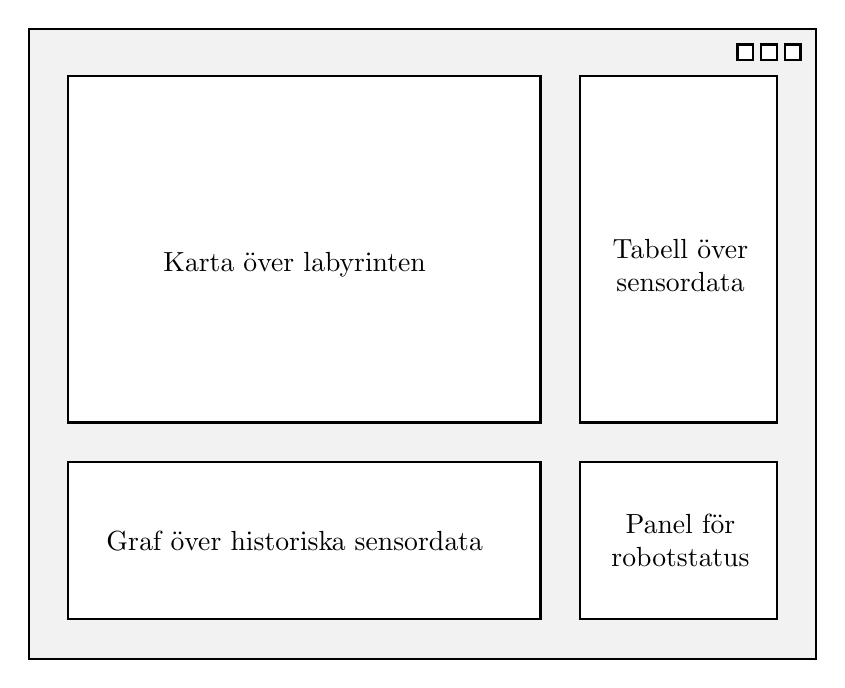
\begin{tikzpicture}[scale=1,rotate=0]
		
	%Frame
	\draw[thick, draw=black, fill=gray!10] (0,0) rectangle (10,8);

	%Exit and minimize
	\draw[thick, draw=black, fill=white] (9.0,7.6) rectangle (9.2,7.8);
	\draw[thick, draw=black, fill=white] (9.3,7.6) rectangle (9.5,7.8);
	\draw[thick, draw=black, fill=white] (9.6,7.6) rectangle (9.8,7.8);
	
	%Map
	\draw[thick, draw=black, fill=white] (0.5,3) rectangle (6.5,7.4);
	\draw  node[left, align=center, text width=5cm] at (6,5) {Karta över labyrinten};
	
	%Table
	\draw[thick, draw=black, fill=white] (7, 3) rectangle (9.5,7.4);
	\draw  node[left, align=center, text width=2cm] at (9.4,5) {Tabell över sensordata};
	
	
	%Graph
	\draw[thick, draw=black, fill=white] (0.5,0.5) rectangle (6.5,2.5);
	\draw  node[left, align=center, text width=5cm] at (6,1.5) {Graf över \mbox{historiska} sensordata};
	
	%Buttons
	\draw[thick, draw=black, fill=white] (7,0.5) rectangle (9.5,2.5);
	\draw  node[left, align=center, text width=2cm] at (9.4,1.5) {Panel för robotstatus};
	
	
	\end{tikzpicture}
	
\end{document}}
	\caption{Datormodulens GUI \label{datormodul:software}}	
\end{figure}

Kartan över labyrinten ritas successivt upp modulvis under robotens färd, och uppdateras alltså efter varje förflyttning till en ny banmodul. I det fall att datorn kopplar upp till roboten efter påbörjad körning skickas all den hittills lagrade kartdatan direkt, varpå kartan sedan uppdateras som beskrivet ovan. Kartan presenteras sedan ur ett fågelperspektiv. I första hand ritas kartan i två dimensioner och i mån av tid utvecklas en tredimensionell karta där roboten följs ur ett tredjepersons-perspektiv. 

Tabellen över sensordata skriver ut informationen från den senaste kommunikationen med huvudmodulen. Kommunikationen består av sensorvärden som huvudmodulen har tagit del av från sensormodulen, som skickas till datormodulen ett fåtal gånger per sekund. Eftersom sensormodulen konverterar de analoga sensor-spänningarna till SI-enheter presenterar tabell-rutan avstånd och vinklar istället för de faktiska spänningsnivåerna. 

Grafen över historiska sensordata tar del av samma information som tabellen, men ritar även ut tidigare data i form av en graf. Denna ruta används främst för felsökning och ger ett tidsperspektiv till sensordatan.

Panelen för knappar visar vilken knappkombination från tangentbordet som är aktiv. Tabell \ref{datormodul:combinations} visar möjliga knappkombinationer och dess översättning till styrkommando. Panelen fyller i de knappar som hålls nere och varnar ifall en knappkombination är otillåten, exempelvis ifall \mbox{$\leftarrow$ och $\rightarrow$} trycks samtidigt.

\begin{longtable}{|p{.05\linewidth} p{.05\linewidth} p{.05\linewidth} p{.05\linewidth} c l|}
	\multicolumn{4}{c}{\textbf{Knapptryckning}} & & \multicolumn{1}{l}{\textbf{Översättning}} 	\\ \nobreakhline\nobreakhline 
	$\uparrow$ &  				&  				& 				& = & Kör framåt 				\\ \nobreakhline 
	$\uparrow$ & $\leftarrow$	&				&				& = & Kör framåt vänster 		\\ \nobreakhline 
	$\uparrow$ &				& $\rightarrow$	&				& = & Kör framåt höger 			\\ \nobreakhline 
			   & $\leftarrow$	&				&				& = & Rotera medurs 			\\ \nobreakhline
			   &				& $\rightarrow$	&				& = & Rotera moturs 			\\ \nobreakhline
			   & $\leftarrow$	&				& $\downarrow$	& = & Kör bakåt vänster 		\\ \nobreakhline
			   &				& $\rightarrow$ & $\downarrow$	& = & Kör bakåt höger 			\\ \nobreakhline
			   &				&				& $\downarrow$	& = & Kör bakåt 				\\ \nobreakhline
	\caption{Knapptryckningar och dess översättning} \label{datormodul:combinations}
\end{longtable}



\subsection{Hårdvara}
Datormodulen kräver en dator kompatibel med Java och Bluetooth\textsuperscript{\circledR}. 

\subsection{Mjukvara}
Gränssnittet programmeras i Java SE 7 och körs i Java Runtime Environment. Valet av programmeringsspråk faller på Java eftersom samma mjukvara ska köras på Windows, OSX och Linux. Kommunikationen via Bluetooth\textsuperscript{\circledR} sker med hjälp av ett existerande Bluetooth\textsuperscript{\circledR}-API utvecklat av Oracle för Java. 

Swing och AWT används för att ge användaren ett grafiskt gränssnitt. Själva huvudklassen är centrerad kring Bluetooth\textsuperscript{\circledR}-kommunikationen och loopar i takt med att en ny sändning har skickats eller mottagits. 

\pagebreak
\section{Intermodulär kommunikation}\label{Intermodulär kommunikation}
För kommunikation mellan de olika modulerna kommer en I\textsuperscript{2}C-buss och Bluetooth\textsuperscript{\circledR} användas. 

\subsection{I\textsuperscript{2}C-buss}

För att kommunicera mellan de olika modulerna kommer den två-trådade I\textsuperscript{2}C-bussen att användas. Då modulerna i huvudsak kommer bestå av processorn \verb+ATmega16+ kommer allt vara kopplat till samma buss. Detta för att \verb+ATmega16+ enbart har en uppsättning av de ingångar som krävs, SCL och SDA. Eftersom mycket av tänkandet ligger i huvudmodulen får den master-status. Resterade blir slavar då informationen som ska mellan sensormodulen och styrmodulen även behövs i huvudmodulen.

\subsubsection{Slavadresser}
I tabell \ref{slavAdress} listas den adress respektive modul ska konfigureras med. 

\begin{center}
\begin{longtable}{|l|l|} \hline
\textbf{Modul} & \textbf{Adress}\\ \hline 
Huvudmodul & 1100100 \\ \hline
Sensormodul & 1100101 \\ \hline
Styrmodul & 1100110\\ \hline
\caption{Modulernas adresser för kommunikation över I\textsuperscript{2}C-bussen}
\label{slavAdress}
\end{longtable}
\end{center}


\subsection{Bluetooth\textsuperscript{\circledR}-kommunikation}
För dataöverföring via Bluetooth\textsuperscript{\circledR} kommer FireFly-modulen användas. Robotens enhet kommer vara kopplad till huvudmodulens processor. Överföringen sker seriellt med protokoll enligt figur \ref{bluetooth}.

\begin{figure}[htbp]
\centering
\noindent\resizebox{.8\linewidth}{!}{
	\documentclass[crop,tikz]{standalone}
\usepackage{tikz}
\usetikzlibrary{calc}
\usetikzlibrary{positioning}
\begin{document}
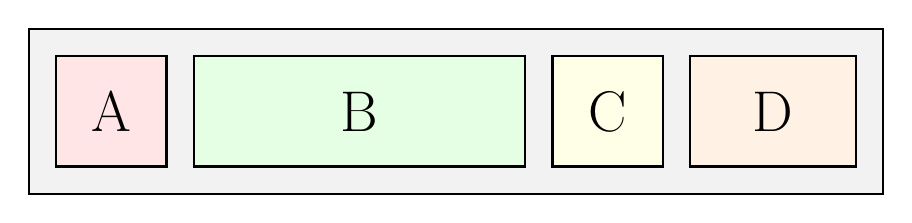
\begin{tikzpicture}[scale=0.07,rotate=0]
		
	%Frame
	\draw[thick, draw=black, fill=gray!10] (0,0) rectangle (155,30);

	%Segments
	%A
	\draw[thick, draw=black, fill=red!10] (5,5) rectangle (25,25);
	\node at (15,15) {\huge A};
	
	%B
	\draw[thick, draw=black, fill=green!10] (30,5) rectangle (90,25);
	\node at (60,15) {\huge B};

	%C
	\draw[thick, draw=black, fill=yellow!10] (95,5) rectangle (115,25);
	\node at (105,15) {\huge C};

	%D
	\draw[thick, draw=black, fill=orange!10] (120,5) rectangle (150,25);
	\node at (135,15) {\huge D};
	
\end{tikzpicture}
\end{document}
}
	\caption{Protokoll för överföring mellan huvud- och datormodul \label{bluetooth}}	
\end{figure}

Respektive segment motsvarar följande:
\begin{itemize}
	\item A - Startbit
	\item B - Informationsbitar (åtta bitar)
	\item C - Paritetsbit
	\item D - Slutbit (en eller två stycken)
\end{itemize}

För att initiera kontakt används så kallade handskakningssignaler för att avgöra om vardera ände är redo att skicka respektive ta emot.

\subsection{Informationsflöde}
I figur \ref{informationFlow} visualiseras informationsflödet. Där anges mottagare och sändare samt vilken typ av information som går mellan dem.

\begin{figure}[htbp]
\centering
\noindent\resizebox{.8\linewidth}{!}{
	\documentclass[border=10px]{standalone}
\usepackage{tikz}
\usetikzlibrary{patterns}
\usetikzlibrary{shapes.geometric}
\usetikzlibrary{shapes.arrows}
\usepackage{amssymb}
\usetikzlibrary{calc}
\usepackage{verbatim}

\pagestyle{empty}
\begin{document}

\tikzstyle{decision} = [diamond, draw,
    text width=4em, text badly centered, node distance=3cm, inner sep=0pt]
    
\tikzstyle{block} = [rectangle, draw,
    text width=7em, text centered, rounded corners, minimum height=4em]
	
\begin{tikzpicture}[scale=1]

%http://www.texample.net/tikz/examples/simple-flow-chart/

\node (robot) at (-1,4.2) {\verb+Robot+};
\node[block] (styr) at (0,0) {Styrmodul};
\node[block] (sensor) at (3.5,3) {Sensormodul};
\node[block] (huvud) at (7,0) {Huvudmodul};
\draw[dashed] (-1.65,-2) rectangle (8.6,4);

\node[block] (dator) at (15,0) {Datormodul};


\draw[-latex, bend left] (huvud) edge node[above]{Kartinformation} node[below]{Sensordata}(dator);
\draw[-latex, bend left] (dator) edge node[below]{Styrkommandon} node[above]{Styrinställningar} (huvud);

\draw[-latex, bend left] (huvud) edge node[below]{Sensordata}(styr);
\draw[-latex] (huvud) edge node[above]{Styrkommandon} (styr);
\draw[-latex, bend right] (huvud) edge node[above]{Styrinställningar} (styr);

\draw[->] (sensor.east) -| node[above]{Sensordata}(huvud.north);
	\end{tikzpicture}
	
\end{document}}
	\caption{Schema över informationsflödet\label{informationFlow}}	
\end{figure}

\subsubsection{Kommunikationsprotokoll - styrkommandon}
Följande protokoll används för att skicka styrkommandon (gäller både för datormodul $\rightarrow$ huvudmodul och huvudmodul $\rightarrow$ styrmodul):

\begin{figure}[htbp]
\centering
\noindent\resizebox{.8\linewidth}{!}{
	\documentclass[crop,tikz]{standalone}
\usepackage{tikz}
\usetikzlibrary{calc}
\usetikzlibrary{positioning}
\begin{document}
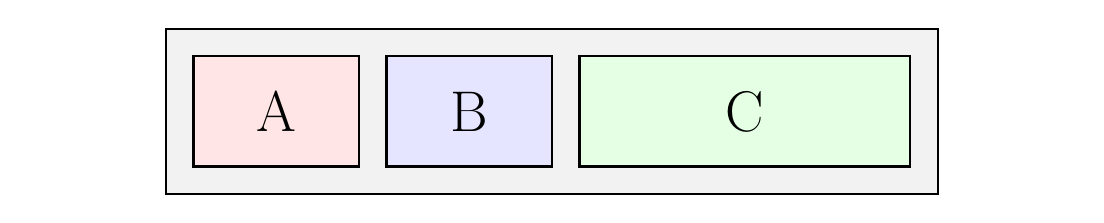
\begin{tikzpicture}[scale=0.07,rotate=0]
	
	%Background
	\draw[draw=white, fill=white] (0,0) rectangle (190,30);
		
	%Frame
	\draw[thick, draw=black, fill=gray!10] (25,0) rectangle (165,30);

	%Segments
	%A
	\draw[thick, draw=black, fill=red!10] (30,5) rectangle (60,25);
	\node at (45,15) {\huge A};

	%B
	\draw[thick, draw=black, fill=blue!10] (65,5) rectangle (95,25);
	\node at (80,15) {\huge B};
	
	%C
	\draw[thick, draw=black, fill=green!10] (100,5) rectangle (160,25);
	\node at (130,15) {\huge C};
	

	
\end{tikzpicture}
\end{document}}
	\caption{Protokoll för överföring av styrkommandon\label{styrdata}}	
\end{figure}

Respektive segment motsvarar följande: 
\begin{itemize}
	\item A - Startbit
	\item B (Bit x-y) - Definierar om ett körkommando eller ett sensorvärde skickas.
	\item C (Bit x-y) - Definierar vilket kommando eller vilken typ av värde som skickas.
	\item D (Bit x-y) - Hastighet (om körkommando och inte reglering), sträcka/vinkel (om körkommando och reglering) eller värde (om sensorvärde).
	\item E - Slutbit
\end{itemize}

\subsubsection{Kommunikationsprotokoll - kartinformation}
Huvudmodulen kommer för varje ny kartmodul skicka data till datormodulen som ritar upp den nya informationen grafiskt. 

Varje korsning kommer att representeras som en nod och vägarna däremellan som bågar. För att så enkelt som möjligt överföra denna information från huvudmodulen till datormodulen kommer varje nod att representeras enligt protokollet nedan:

 \begin{figure}[H]
\centering
\noindent\resizebox{.8\linewidth}{!}{
	\documentclass[crop,tikz]{standalone}
\usepackage{tikz}
\usetikzlibrary{calc}
\usetikzlibrary{positioning}
\begin{document}
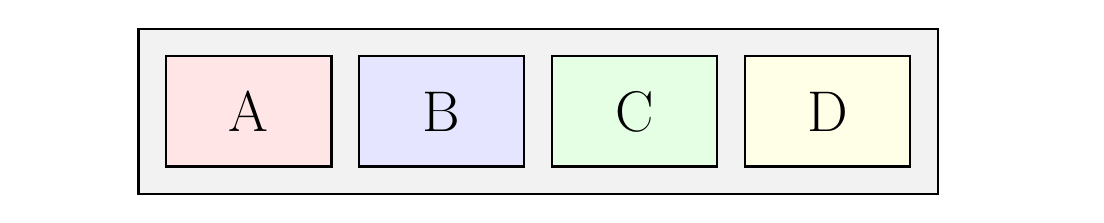
\begin{tikzpicture}[scale=0.07,rotate=0]
		
	%Background
	\draw[draw=white, fill=white] (0,0) rectangle (190,30);	
		
	%Frame
	\draw[thick, draw=black, fill=gray!10] (20,0) rectangle (165,30);

	%Segments
	%A
	\draw[thick, draw=black, fill=red!10] (25,5) rectangle (55,25);
	\node at (40,15) {\huge A};

	%B
	\draw[thick, draw=black, fill=blue!10] (60,5) rectangle (90,25);
	\node at (75,15) {\huge B};
	
	%C
	\draw[thick, draw=black, fill=green!10] (95,5) rectangle (125,25);
	\node at (110,15) {\huge C};
	
	%D
	\draw[thick, draw=black, fill=yellow!10] (130,5) rectangle (160,25);
	\node at (145,15) {\huge D};
	
\end{tikzpicture}
\end{document}}
	\caption{Protokoll för överföring av kartdata \label{kartdata}}	
\end{figure} 

Respektive segment motsvarar följande: 
\begin{itemize}
	\item A - Startbit
	\item B (Bit 0-3) - Motsvarar nodens x-koordinat (0-15)
	\item C (Bit 4-7) - Motsvarar nodens y-koordinat (0-15)
	\item D (Bit 8-11) - Representerar väggar kring noden (1 = vägg, 0 = ingen vägg) i nordlig, västlig, sydlig och östlig riktning (b8 = N, b9 = W, b10 = S, b11 = E).
	\item E - Slutbit
\end{itemize}

\subsubsection{Kommunikationsprotokoll - sensordata}
Sensordata skickas enligt följande protokoll:

 \begin{figure}[H]
\centering
\noindent\resizebox{.8\linewidth}{!}{
	\documentclass[crop,tikz]{standalone}
\usepackage{tikz}
\usetikzlibrary{calc}
\usetikzlibrary{positioning}
\begin{document}
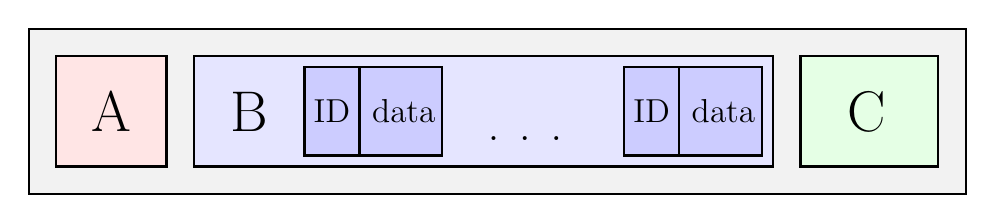
\begin{tikzpicture}[scale=0.07,rotate=0]
		
	%Frame
	\draw[thick, draw=black, fill=gray!10] (0,0) rectangle (170,30);

	%Segments
	%A
	\draw[thick, draw=black, fill=red!10] (5,5) rectangle (25,25);
	\node at (15,15) {\huge A};

	%B
	\draw[thick, draw=black, fill=blue!10] (30,5) rectangle (135,25);
	\node at (40,15) {\huge B};
	
	%B1
	\draw[thick, draw=black, fill=blue!20] (50,7) rectangle (60,23);
	\draw[thick, draw=black, fill=blue!20] (60,7) rectangle (75,23);
	\node at (55,15) {\large ID};
	\node at (68,15) {\large data};
	
	\node at (90,10) {\LARGE . . .};
	
	%Bn
	\draw[thick, draw=black, fill=blue!20] (118,7) rectangle (133,23);
	\draw[thick, draw=black, fill=blue!20] (108,7) rectangle (118,23);
	\node at (113,15) {\large ID};
	\node at (126,15) {\large data};

	%C
	\draw[thick, draw=black, fill=green!10] (140,5) rectangle (165,25);
	\node at (152,15) {\huge C};
	
\end{tikzpicture}
\end{document}}
	\caption{Protokoll för överföring av sensordata\label{sensordata}}	
\end{figure} 

Respektive segment motsvarar följande: 
\begin{itemize}
	\item A - Startbit
	\item B - Sensordatapaket
	\item E - Slutbit
\end{itemize}

Sensordatapaketet består av ett antal sensorvärden som skickas tillsammans med ett ID, för att identifiera vilken sensor värdet tillhör. Beroende på vilken styrmod roboten befinner sig i skickas olika sensorvärden. En tabell över vilka sensorvärden som skickas i respektive styrmod och en över de olika sensorernas ID finns nedan.

\begin{table}
\begin{tabular}[l]{| l | p{0.7\linewidth} |} \hline
\textbf{Styrmod} & \textbf{Skickade sensordata} \\ \hline 
Körning rakt fram i korridor & Avstånd till främre väggen $s$, avstånd till sidoväggen $z$, vinkelhastighet $\omega$, vinkel i förhållande till väggen $(\theta-\gamma)$ \\ \hline
Rotation & Vinkelhastighet $\omega$ \\ \hline
Körning i öppen yta & \textit{fylls på efter förstudien} \\ \hline
%\caption{Tabell över de olika styrmoderna. För förtydligande av variabler, se figur \ref{robotwall}, s.\pageref{robotwall}}
\end{tabular}
\end{table}


\begin{longtable}[l]{| l | l | c |} \hline
\textbf{ID} & \textbf{Sensor} & \textbf{Enhet} \\ \hline 
0 & IR-sensor höger-fram & cm \\ \hline
1 & IR-sensor vänster-fram  & cm \\ \hline
2 & IR-sensor höger-bak  & cm  \\ \hline
3 & IR-sensor vänster-bak  &  cm \\ \hline
4 & Lasersensor & cm  \\ \hline
5 & Rörelse i x-led & m/s\textsuperscript{2} \\ \hline
6 & Rörelse i y-led & m/s\textsuperscript{2} \\ \hline
7 & Rörelse i z-led & m/s\textsuperscript{2} \\ \hline
8 & Rotation kring x-axeln & rad/s \\ \hline
9 & Rotation kring y-axeln & rad/s \\ \hline
10 & Rotation kring z-axeln & rad/s \\ \hline
11 & IR-sensor för mål & cm \\ \hline
\caption{Tabell över sensorerna}
\end{longtable}


\pagebreak
\section{Implementering}
Här beskrivs hur robotens delar ska implementeras. 


\subsection{Fysisk design}
Roboten kommer bestå av 3 virkort där varje virkort motsvarar en av robotens tre moduler. Detta för att enkelt kunna se modulariteten och jobba med olika moduler samtidigt.

\subsection{Testning och feedback}
I början av utvecklingen av roboten färdigställs I\textsuperscript{2}C-bussen för att tidigt ha kommunikationen klar så att denna kan testas kontinuerligt under projektets gång. Hårdvara och mjukvara bör testas för sig först och sedan ihop för att lättare felsöka. Hjälp för testning är exempelvis Atmel Studio och JTAG ICE för on-chip debugging eller logikanalysator. Varje delmodul testas med simulerad data för att se att den fungerar som önskat. För att enklare kunna se vad som händer kan en extern klocka kopplas till processorn för att få tillräckligt låg frekvens. Optimalt är att varje delfunktion av roboten testas så fort den är klar för att kunna säkerställa att den fungerar innan utvecklingsarbetet fortgår.  

Inom utvecklingsarbetet för varje aktivitet hanteras också eventuell felhantering. Denna felhantering görs på alla eventuella problem som kan tänkas uppstå. Till processorn kan exempelvis en LED-lampa kopplas för att få feedback att något gått fel. I programvara i datorn är det lämpligt att använda sig av en körlogg för att kunna gå tillbaka och se vilken data som skickades när för att smidigt kunna se var och när något gick fel om det gjorde det. Den LCD-display som är kopplad på styrmodulen ska förutom sensordata även kunna visa styrkommandon för att kunna se vad som händer vid körning.

\subsection{Sampling}
Det som begränsar tiden mellan samplingar av sensordata är hur lång tid A/D omvandlingen tar för den data som tar längst tid att omvandla. Sampling bör ske så ofta som möjligt för så bra värde som möjligt så att styrmodulen kan få uppdaterade värden skickade till sig. Sampling kommer ske med frekvens mellan 10-20 Hz för att hinna med omvandling av IR-sensorernas data. 


\pagebreak
\addcontentsline{toc}{section}{Referenser}
\bibliographystyle{ieeetr}
\bibliography{references}

\end{flushleft}

\end{document}